\begin{document}
%\pagenumbering{Roman}

%---------------------------------------------------------------------------
% TITLE PAGE
%---------------------------------------------------------------------------

% DO NOT REMOVE SPACES BETWEEN LINES!

\let\temp\newpage
\let\newpage\relax
\begin{titlepage}

\AddToShipoutPicture*{\BackgroundPic}

\hspace{-0.6cm}
\includegraphics[width=0.6\textwidth]{logo_polimi_ing_indinf.eps}

\vspace{-0.2cm}
\Large{\textbf{\color{bluePoli}{\title}}}\\
\hspace*{\fill}

\vspace{-0.2cm}
\fontsize{0.3cm}{0.5cm}\selectfont \bfseries \textsc{\color{bluePoli} MSc in \course}\\
\hspace*{\fill}

\vspace{-0.2cm}
\fontsize{0.3cm}{0.5cm} \selectfont \bfseries Authors:\par
\vspace{0.2cm} \hspace{0.3cm} \textsc{\textbf{\authors}}\\
\hspace*{\fill}

\fontsize{0.3cm}{0.5cm}\selectfont \bfseries Professor: \textsc{\textbf{\professor}}\\
\hspace*{\fill}

% if only ONE co-advisor is present:
%\vspace{-0.4cm}
%\fontsize{0.3cm}{0.5cm}\selectfont \bfseries Co-advisor: %\textsc{\textbf{\firstcoadvisor}}\\
% if more than one co-advisors are present:
%\vspace{-0.4cm}
%\fontsize{0.3cm}{0.5cm}\selectfont \bfseries Co-advisors: \textsc{\textbf{\firstcoadvisor}}\textsc{\textbf{\secondcoadvisor}}\\

\vspace{-0.4cm}
\fontsize{0.3cm}{0.5cm}\selectfont \bfseries Academic year: \textsc{\textbf{\YEAR}}

\small \normalfont

\vspace{11pt}

\centerline{\rule{1.0\textwidth}{0.4pt}}

\vspace{15pt}

\end{titlepage}
\let\newpage\temp

\thispagestyle{plain} % In order to not show the header in the first page

%\vspace*{20mm}
%\begin{abstract}
\addcontentsline{toc}{chapter}{Abstract}
\vspace*{10mm}

\lipsum[1]

\end{abstract}

%---------------------------------------------------------------------------
% INDEX
%---------------------------------------------------------------------------

{\let\clearpage\relax
\vspace*{10mm}
\hypersetup{linkcolor=black}
\small
\tableofcontents}
\clearpage

%{\hypersetup{linkcolor=black}\listoftables}

%{\hypersetup{linkcolor=black}\listoffigures}

%---------------------------------------------------------------------------
% BEGINNING OF THE WRITTEN PART
%---------------------------------------------------------------------------

%\setcounter{page}{1}
%\pagenumbering{arabic}

\chapter{Interplanetary mission}
%\section{Symbols}
\label{sec:symbols}
%\setcounter{subsection}{2}
\newsavebox\ltmcbox
\renewcommand{\arraystretch}{1.2}
\renewcommand\tabularxcolumn[1]{m{#1}}

\begin{multicols}{2}
	\raggedcolumns

	\subsubsection{Analisi della missione}
	\vspace{-10pt}
	\small
	\setbox\ltmcbox\vbox{
	\makeatletter\col@number\@ne
	\begin{xltabular}{\linewidth}{cc>{\raggedright\arraybackslash}X}
		$\bm{A_e}$ & $[m^2]$ & area di efflusso totale \\
		$\bm{\phi}$ & $[rad]$ & angolo di traiettoria del razzo
	\end{xltabular}
	\unskip
	\unpenalty
	\unpenalty}
	\unvbox\ltmcbox

	\subsubsection{Analisi della missione 2}
	\vspace{-10pt}
	\small
	\setbox\ltmcbox\vbox{
	\makeatletter\col@number\@ne
	\begin{xltabular}{\linewidth}{cc>{\raggedright\arraybackslash}X}
		$\bm{A_e}$ & $[m^2]$ & area di efflusso totale \\
		$\bm{\phi}$ & $[rad]$ & angolo di traiettoria del razzo
	\end{xltabular}
	\unskip
	\unpenalty
	\unpenalty}
	\unvbox\ltmcbox

\end{multicols}
\subsection{Introduction}
\label{subsec:introduction}

\subsubsection{Description of the problem}
\label{subsubsec:description}
The first part of the assignment aims at designing an interplanetary transfer from Mars to asteroid 1036 Ganymede exploiting a powered gravity assist on Earth. The problem is analyzed through the patched conics method, without considering the injection and arrival hyperbolas. The initial and final velocity vector of the satellite are assumed to be the same of the respective celestial body. The two heliocentric legs are calculated through the Lambert problem. The trajectory is selected with the only criteria of minimizing the cost of the mission, assessed through the total $\Delta V$. The latter is computed by summing different contributions:

\begin{equation}
    \Delta V_{tot}= \Delta V_1 + \Delta V_2 + \Delta V_3
\end{equation}

Where the three terms are defined as:
\begin{itemize}
    [wide,itemsep=3pt,topsep=3pt]
    \item $\Delta V_1$ injection in the first heliocentric leg;
    \item $\Delta V_2$ exit from the second heliocentric leg;
    \item $\Delta V_3$ impulse given by the engine at pericentre of hyperbola fly-by;
\end{itemize}


All the manoeuvres are assumed to be impulsive, i.e. they change only the velocity vector of the spacecraft, mantaining invariated the position vector. Note that $\Delta V_{1}$ and $\Delta V_{2}$ are related to heliocentric velocities, while $\Delta V_{3}$ is calculated through relative geocentric velocities. 

For each manoeuvre the cost is computed as:

\begin{equation}
    \Delta V_i= \lVert \boldsymbol{V_{+,i}} - \boldsymbol{V_{-,i}} \rVert
\end{equation}


\subsubsection{Assigned data and constraints}
\label{subsubsec:data_constraints}
A few constraints were considered:
\begin{itemize}
    [wide,itemsep=3pt,topsep=3pt]
    \item earliest departure date $t_{min,dep} = \left[01/01/2028 \;\; 00:00:00\right]$ in Gregorian calendar
    \item latest arrival date $t_{max,arr} = \left[01/01/2058 \;\; 00:00:00\right]$ in Gregorian calendar
    \item time of flights of the two heliocentric arcs must be greater than the associated parabolic time
    \item minimum pericentre radius of the fly-by hyperbola $r_p = r_E + 500 \; km$
    \item single-revolution Lambert problem was considered
    \item reasonable total time of the mission
\end{itemize}

Note that the constraint on the pericentre radius of the fly-by is considered both for avoid impact on Earth and to prevent undesired atmoshperic drag effects. 




\section{Algorithms description}
\label{sec:algo_description}

The targeting problem previously defined can be seen as an optimization problem with three degrees of freedom (DOFs). Indeed, once the departing date and the two times of flight of the heliocentric legs are chosen, both the Lambert's arcs and the fly-by hyperbola are fully defined.  
Regarding the formulation of the Lambert's problem, it requires the knowledge of the initial and final position and also the imposed time of flight between them. For two Lambert's arcs it would be needed a total of six DOFs, but this quantities are dependant one to each other:
\begin{itemize}
    [wide,itemsep=3pt,topsep=3pt]
    \item the final position vector of the first arc corresponds to the initial position of the second one;
    \item the initial date for the departing on the second arc corresponds the arrival date on the first arc;
    \item fixing the first Lambert's arc, the final position and arrival date for the second Lambert's arc are related through the analytical ephemerides.
\end{itemize}

Once the two heliocentric legs are determined, the powered gravity assist follows as the geocentric velocity vectors are known.

The method implemented to solve the optimization problem is the \textbf{brute force algorithm} refined with the \textbf{gradient descent algorithm}. Then, to validate the results, the \textbf{brute force algorithm} has been used solely with a more dense search grid in a reasonable domain. 

\subsection{Refined brute force algorithm}
\label{subsec:brute_force_algo}

The presented \autoref{alg:brute} is reliable, yet  computationally demanding since the research of the minimum is performed through a triple-nested \textit{for} loop. The time of the execution highly depends on the refinement chosen for the three selected periods of time. From this considerations and also noticing that the function to minimize presents high irregularities, it is clear that narrow time windows can help in the overall research. Moreover, with this last observation, it is possible to use a less fine grid of research, since it is reasonable to think that the function will present less irregularities.

\begin{algorithm}
    \caption{Bruteforce algorithm} \label{alg:brute}
    \begin{algorithmic}
    \Require $T_{dep}, \Delta T_{1}, \Delta T_{2}$
    \State $\Delta V_{min} = 10^{10}$
    \For{$i$ in $T_{dep}$}
        \For{$j$ in $\Delta T_{1}$} 
            \State Calculate $T_{fly-by}$, first Lambert's arc, Mars' velocity at $T_{dep}$ and  $\Delta V_1$
            \For{$k$ in $\Delta T_{2}$}
                \State Calculate $T_{arr}$, second Lambert's arc, Asteroid's velocity at $T_{arr}$, $\Delta V_2$, $\Delta V_3$, $\Delta V_{tot}$
                \If{$\Delta v_{tot} < \Delta v_{min}$ and $r_p > r_{Earth} + 500 \; km$}
                \State $\Delta v_{min} = \Delta v_{tot}$
                \State $T_{dep,min} = T_{dep} $;   $T_{fb,min}  = T_{fb}$;   $T_{arr,min} = T_{arr}$
                \EndIf
            \EndFor
        \EndFor
    \EndFor
\State Minimize cost using \textit{fminunc} with initial guess  $\left(T_{dep,min};T_{fb,min};T_{arr,min} \right)$
\\
\Return $\Delta V_{min}$; $T_{dep,min}$; $T_{fb,min}$; $T_{arr,min}$
    \end{algorithmic}
\end{algorithm}

As a consequence, it was decided to perform a physical analysis (\autoref{sec:time_red}) in order to wisely reduce the time domains for departure, fly-by and arrival. The idea of \autoref{alg:brute} is that, once this reduction is performed, the brute-force search can be carried out on a small but refined grid. To speed up the process and refine the solution, \textit{fminunc} of \textit{MATLAB} was used. The selected initial guess is the outcome of the brute force research.

In order to completely validate the results, the robustness of the brute force algorithm has been exploited. Referring to \autoref{alg:brute}, \textit{fminunc} was removed after the for-loop search and the research grid was refined. Moreover, with this computation it is possible to validate the time reduction analyzed in \autoref{sec:time_red}.
\subsection{Reduction of the time windows}
\label{subsec:time_red}

\subsubsection{Resonance period analysis}
\label{subsubsec:res_period}

\subsubsection{Cost-plot analysis}
\label{subsubsec:cost_plot_analysis}

\subsubsection{Final time window selection}
\label{subsubsec:final_window}
\section{Conclusion and results}
\label{sec:conclusion}

It was then used \autoref{alg:brute} in the time domain selected at the end of \autoref{subsec:cost_plot_analysis},  using 40 elements for each array. The obtained results in terms of cost and dates are reported in the following tables:

\vspace{0.5cm}

\begin{minipage}{0.5\linewidth}
    \centering
    \captionsetup{type=table}
    \begin{tabular}{|c|c|c|c|}
        \hline
        $\Delta V_1 \, [km/s]$ & $\Delta V_2 \, [km/s]$ & $\Delta V_3 \, [km/s]$ & $\Delta V_{tot} \, [km/s]$\\
        \hline
        $4.0813$ & $3.3130$ & $2.7715 \cdot 10^{-6}$ & $7.3942$\\
        \hline
    \end{tabular}
    \caption{Costs $\Delta V$ of the optimal mission}
    \label{table:cost_optimal}
\end{minipage}\hfill
\begin{minipage}{0.5\linewidth}
    \centering
    \captionsetup{type=table}
    \begin{tabular}{|c|c|c|}
        \hline
        Dep. Date & Fb. Date & Arr. Date \\
        \hline
        $\left[03/06/2033 \right]$ & $\left[10/02/2034\right]$ & $\left[27/03/2036\right]$ \\
        \hline
    \end{tabular}
    \caption{Optimal mission dates in Gregorian calendar}
    \label{table:date_optimal}
\end{minipage}
\vspace*{5pt}

The obtained results were validated through the pure brute-force algorithm, with a more refined grid of search in the same domain. In particular 100 elements where considered, the data obtained were:

... put the two tables of brute force algorithm

\subsection{Heliocentric legs}
\label{subsec:heliocentric}
The two heliocentric legs associated with the solution computed through \autoref{alg:brute} can be characterized through the keplerian elements shown in \autoref{table:Orb_Par}:
\begin{table}[H]

    \centering
    \begin{tabular}{|c|c|c|c|c|c|c|c|}
    \hline
    Arc &  $a  \ [AU]$ & $e \ [-]$ & $i \ [deg]$ & $\Omega \ [deg]$ & $\omega \ [deg]$ & $\theta_{dep} \ [deg]$ & $\theta_{arr} \ [deg]$ \\
    \hline
    M$\to$E &  $1.1602$ & $0.2870$ & $1.18$ & $321.55$ & $105.97$ & $195.38$ & $74.03$ \\
    \hline
    E$\to$G & $1.9445$ & $0.5029$ & $4.17$ & $141.55$ & $339.91$ & $20.09$ & $231.37$ \\
    \hline
    \end{tabular}
    
    \caption{Heliocentric legs}
    \label{table:Orb_Par} 
\end{table}

\cfig{solar_system.jpg}{Optimal transfer trajectory - planet's dimension not in scale}{solar_system}{0.75}

The two heliocentric legs are displayed in \autoref{fig:solar_system}. The represented positions of Mars, Earth and 1036 Ganymed are respectively at departure, fly-by and arrival. All the orbits are plotted in the Heliocentric ecliptic inertial frame.
\subsection{Gravity assist}
\label{subsec:ga}

Known the incoming and outcoming heliocentric velocities of the spacecraft and the Earth's velocity at the fly-by date, it was possible to completely characterize the two branches of hyperbola in an Earth-centred ecliptic frame. The main parameters of the hyperbola are reported in \autoref{table:ga}:

\begin{table}[H]

    \centering
    \begin{tabular}{|c|c|c|c|c|c|c|c|}
    \hline
    $r_p \ [km]$ &  $\delta _{tot} \ [\deg]$ & $v_{\infty}^{-} \ [km/s]$ & $v_{\infty}^{+} \ [km/s]$ & $e_{-} \ [-]$ & $e_{+} \ [-]$ & $\Delta T_{soi} \ [days]$ & $\Delta V_{helio} \ [km/s]$ \\
    \hline
    $7763.39$ &  $54.8918$ & $7.743439$ & $7.743435$ & $2.167834$ & $2.167833$ & $2.6871$ & $7.1381$ \\
    \hline
    \end{tabular}
    
    \caption{Gravity assist data}
    \label{table:ga} 
\end{table}

It can be noticed that the fly-by hyperbola respect the constraint on the pericentre radius given in \autoref{subsec:data_constraints}. Moreover, the impulse given by the engine at the pericentre (\autoref{table:cost_optimal}) is negligible with respect to the heliocentric fly-by manoeuvre cost, calculated as $\Delta V_{helio} = \lVert\boldsymbol{V_{\infty}^{+} - V_{\infty}^{-}} \rVert$. This confirms the efficiency effect of the examined fly-by. 

The permanence time passed inside the sphere of influence has been computed using the hyperbolic time law. In particular, considering the intersection between the two hyperbolic arcs and the radius of the Earth's sphere of influence (\autoref{eq:soi}), the true anomalies at entry and exit of SOI are computed.

\begin{equation}
    \label{eq:soi}
r_{SOI,E} = r_{S \to E}\left(\frac{M_E}{M_S}\right)^{2/5} = 9.24647 \cdot 10^{5} \ km
\end{equation}













%---------------------------------------------------------------------------

{\let\clearpage\relax
\vspace*{50mm}
\chapter{Planetary mission}}

\section{Introduction}
\label{sec:introduction_cap2}

The PoliMi Space Agency wants to launch a Planetary Explorer Mission, to  perform  Earth Observation. This section carries out relevant orbital analysis and groundtrack estimation while also considering two perturbation models. A modified groundtrack was proposed for a repeating groundtrack, and two propagation methods are used to perform the analysis which are then compared. A comparison between the real data of a satellite and its analytical results obtained with the code model is also performed for model validity.


\subsection{Nominal Orbit}

From the provided orbital parameters this satellite heavily contains geosynchronous orbital characteristics. Hence, the altitude at perigee is chosen as 35786 km \cite{perigee_alt} - where it is possible to see the moon and J2 perturbation effect. $\Omega$ (right ascension of ascending node), $\omega$ (argument of perigee), and $f_0$ (initial true anomaly) are chosen arbitrarily for a simpler analysis.

\begin{table}[ht]
	\centering
	\label{tab:keplerian_elements}
	\begin{tabular}{|c|c|c|c|c|c|}
		\hline
		a [km] & e [-] & i [$\deg$] & $\Omega$ [$\deg$] & $\omega$ [$\deg$] & $h_p$ [km] \\
		\hline
		42159 & 0.0007 & 32.5934 & 0 & 85 & 35786 \\
		\hline
	\end{tabular}
	\caption{Keplerian elements of the orbit}
\end{table}

The unperturbed nominal orbit is propagated as below in the Earth-centered reference frame:

\cfig{nominal_orbit.eps}{Assigned orbit}{nominal_orbit}{0.85}
\section{Groundtrack}
\label{sec:groundtrack}

The satellite's orbit is propagated to compute its groundtrack. The motion of the spacecraft is assumed to be a perturbed two body problem in Cartesian coordinates, described by the equation:

\begin{equation}
	\dot{\mathbf{r}} = -\frac{\mu}{r^3} \mathbf{r} + \mathbf{a}_{\text{perturbation}}
\end{equation}

This is solved using \textit{MATLAB}'s multi-step solver \texttt{ode113} function which is based on the Adams-Bashforth-Moulton method; it's chosen for its high accuracy over an extended period. A relative tolerance of \(1 \times 10^{-12}\) and absolute tolerance of \(1 \times 10^{-12}\) were selected for more precision.
%citation for formula: Curtis


\subsection{Unperturbed Groundtrack}

\subsubsection{Nominal Orbit Groundtrack}

The first required analysis of the ground track is for the nominal orbit considering an unperturbed case, where the $\mathbf{a}_{perturbation}$ in equation is null. The ground track was propagated for a period of 1 orbit of the satellite, 1 day and 10 days, as shown below.

\IVfig{ug1orb.eps}{ug1d.eps}{ug10d.eps}{ugstartend.png}{unpert_grountrack}{
	Ground track of the unperturbed nominal orbit during: (a) 1 orbit; (b) 1 day; (c) 10 days. Ground track path (\reddashedline), Starting point (\textcolor{red}{$\bullet$}), Ending point (\textcolor{red}{$\blacksquare$}).
}{0.9}

The groundtrack of this satellite has formed an “8” shape, a phenomenon known as the figure-eight groundtrack. At geosynchronous altitude, the location after one revolution is the same, and for geostationary  orbits, the satellite always appears to be stationary over one location. The figure “8” occurs because the satellites relative velocity is less and greater, than locations on the Earth as it travels from the ascending node \cite{vallado}.


\subsubsection{Repeating Groundtrack}

For establishing a good communication with the network of ground stations of PoliMi Space Agency, a repeating ground track with a ratio of 1:1 (for each orbit of the spacecraft, Earth has performed 1 revolution) is maintained. Therefore, the period of the repeating ground track orbit is computed. For an unperturbed orbit, the period is only a function of the semi-major axis and can be calculated to get the desired repeating ground track. Both equations are listed below. By extension, the other orbital parameters are kept the same as the nominal orbit. 
	
\begin{equation}
	T_{\text{repeating}} = \frac{1}{1} T_{\text{Earth}} \qquad
	T = 2\pi \sqrt{\frac{a^3}{\mu}} \rightarrow a_{\text{repeating}} = 42166 \; \text{km}
\end{equation}

\twofig{ugro1orb.eps}{ugro4orb.eps}{ground_repetition}{
	Ground track of the unperturbed repeating orbit during: (a) 1 orbit; (b) 4·k=4 orbits. Ground track path (\reddashedline), Starting point (\textcolor{red}{$\bullet$}), Ending point (\textcolor{red}{$\blacksquare$}).
}{0.85}


\subsection{Perturbed Groundtrack}

\subsubsection{Assigned Perturbations}

This project has been assigned with two perturbations: \( J_2 \) effect and Moon perturbation. \( J_2 \) effect consists of a perturbing potential on top of the central gravity field of the Earth. In order to model it, a zonal harmonic potential is used, function of the geocentric distance \( r \) and of the coelevation \( \phi \).

\begin{equation}
	R(r, \phi) = \frac{\mu}{r} \left( -1 + \sum_{n=2}^{\infty} \left( \frac{R_E}{r} \right)^n J_n P_n(\cos\phi) \right)
\end{equation}

Here, \( J_2 \) term is considered for modelling which is correlated to Earth oblateness. The perturbing acceleration due to \( J_2 \) effect is given as:

\begin{equation}
	\mathbf{a}_{J_2} = \frac{3}{2} \frac{J_2 \mu R_E^2}{r^4} \left[ \left( \frac{x}{r} \left( \frac{5z^2}{r^2} - 1 \right) \right) \mathbf{i} + \left( \frac{y}{r} \left( \frac{5z^2}{r^2} - 1 \right) \right) \mathbf{j} + \left( \frac{z}{r} \left( \frac{5z^2}{r^2} - 3 \right) \right) \mathbf{k} \right]
\end{equation}
%citation: Vallado, Curtis

Perturbation due to the moon acting on the orbit is modelled through a two body problem scenario taking into account the force of the moon as a perturbing acceleration. This acceleration is computed from:
\begin{equation}
	\label{eq:moon_perturbation}
	\mathbf{a}_{\text{Moon}} = \mu_{\text{Moon}}
	\left( \frac{\mathbf{r}_{m/s}}{r_{m/s}^3} - \frac{\mathbf{r}_m}{r_m^3} \right)
\end{equation}

where \( \mathbf{r}_{m/s} \) is the vector that goes from the S/C to the moon and \( \mathbf{r}_m \) is the vector that goes from Earth to Moon.

Possible perturbations are charted in \autoref{fig:orbit perturbations}. It is observed that the \( J_2 \) effect (\( C_{2,0} \) in figure) and moon perturbation are one of the primary sources of orbital perturbation. Hence, our models and altitude choice are consistent.   

\cfig{Perturbation chart.png}{Orbit Perturbations from \cite{thesis_chart}}{orbit perturbations}{0.5}


\subsubsection{Nominal and Repeating Groundtrack}

\begin{figure}[H]
	\begin{minipage}{0.48\linewidth}
		\centering
		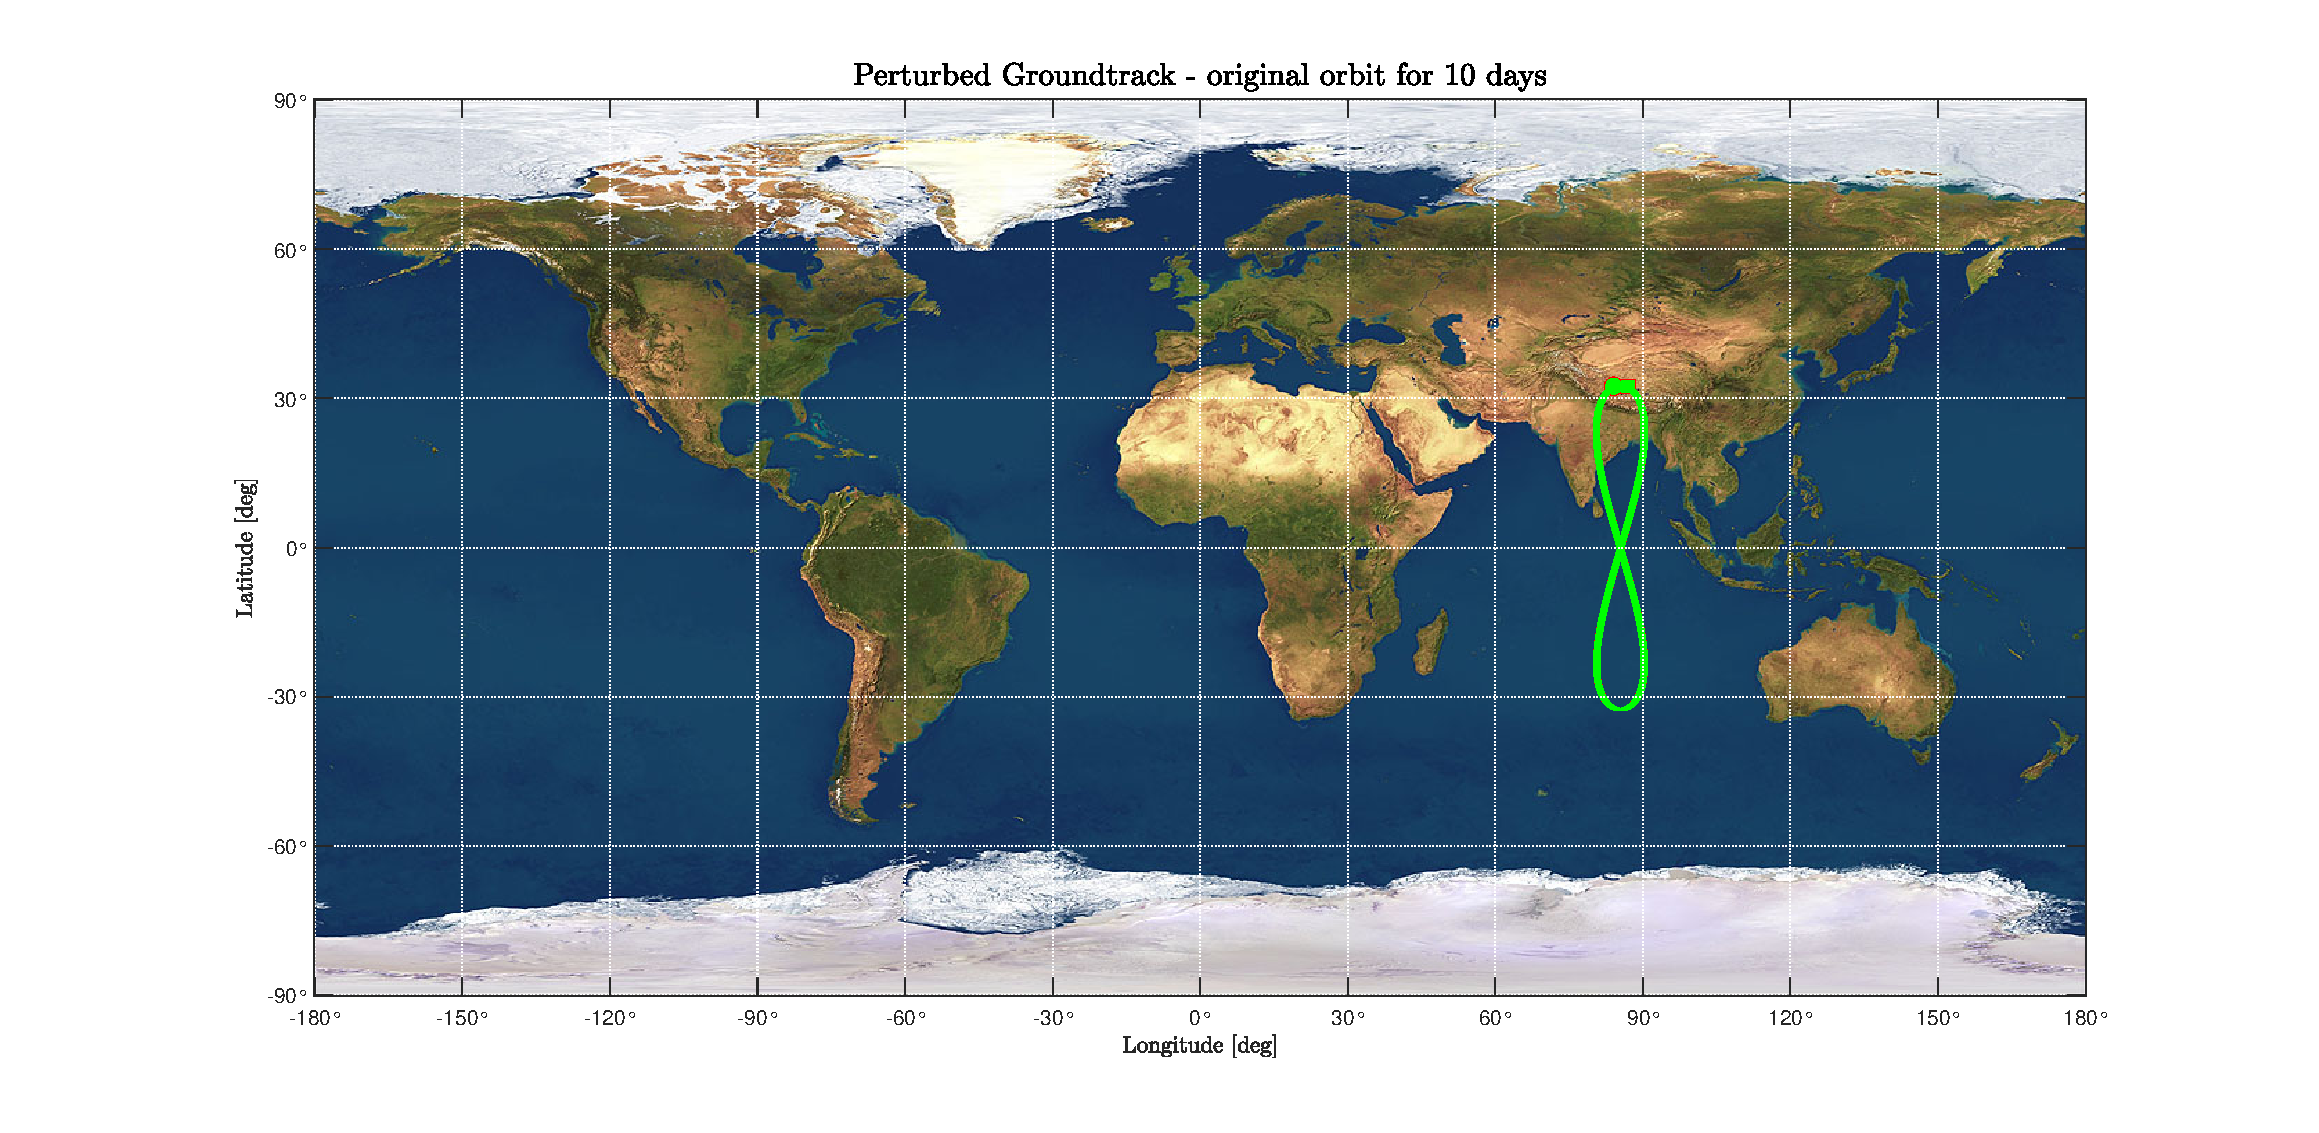
\includegraphics[width=\linewidth]{pg10d.eps}
	\end{minipage}\hfill
	\begin{minipage}{0.48\linewidth}
		\centering
		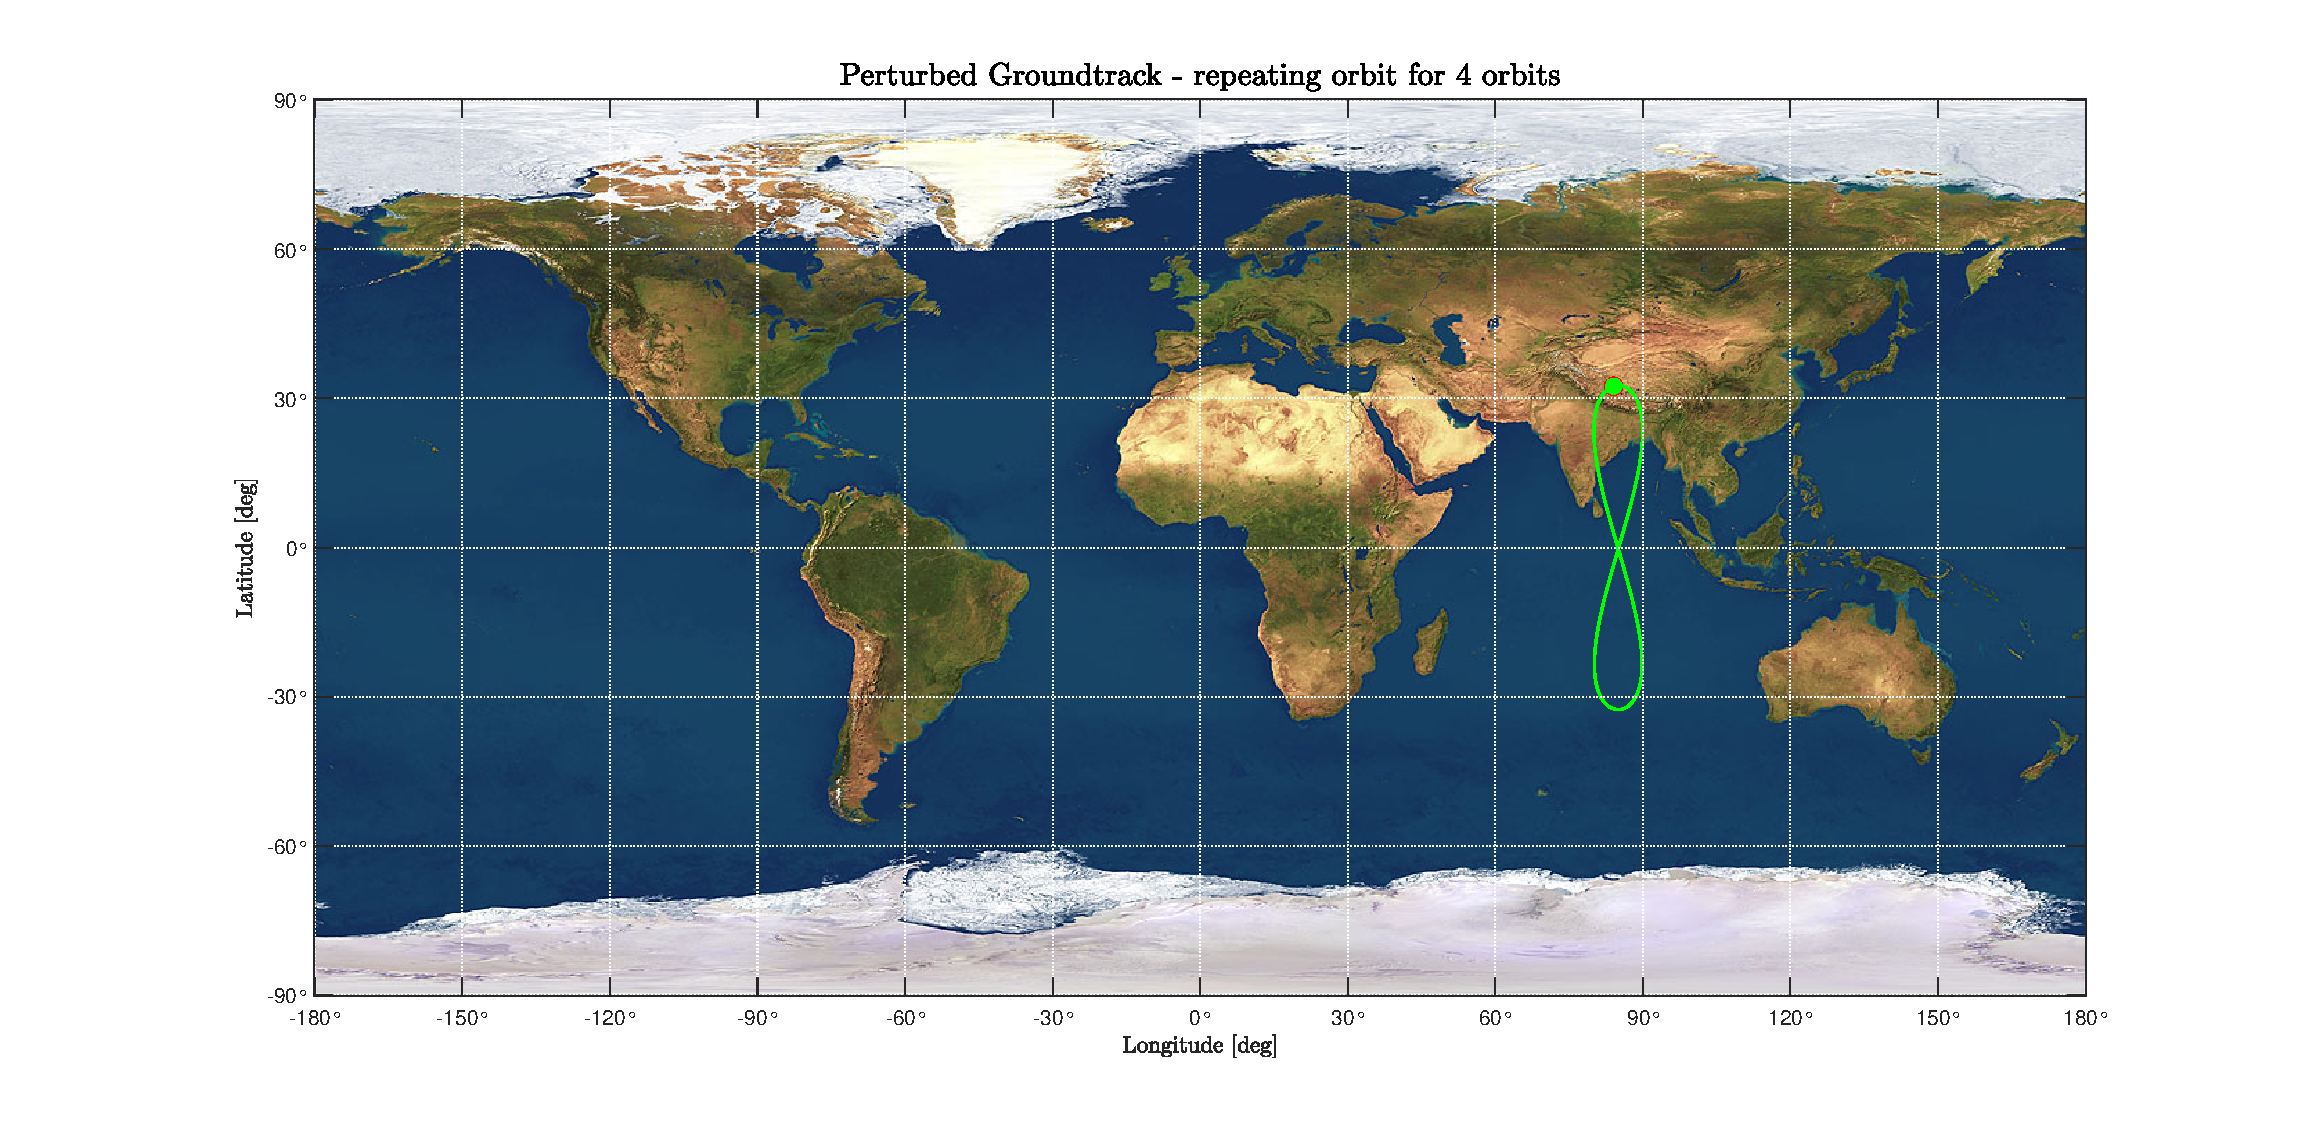
\includegraphics[width=\linewidth]{pgro4orb.eps}
	\end{minipage}
\end{figure}

\cfig{zoompgro4orb.eps}{
	Ground track of the perturbed orbits: (a) Nominal orbit during 10 days; (b) Repeating orbit during 4 orbits; (c) Perturbation effect for repeating orbit. Ground track of unperturbed (\reddashedline), Starting point (\textcolor{red}{$\bullet$}), Ending point (\textcolor{red}{$\blacksquare$}); Ground track of perturbed (\greendashedline), Starting point (\textcolor{green}{$\bullet$}), Ending point (\textcolor{green}{$\blacksquare$}).
}{groundtrack}{0.6}

It is observed that the perturbations have a great impact on the ground track path of the satellite. Both the nominal and repeating orbits get out of phase with relation to the unperturbed case. From \autoref{fig:groundtrack}, the repeating ground track orbit proposed does not work in the presence of assigned perturbations.
\section{Orbit Propagation}
\label{sec:orbit_propagation}

Orbits were propagated using Cartesian coordinates (Newton’s equations of motion), or Keplerian elements (Gauss’ planetary equations). Gauss' equations are presented in the Radial-Transversal-Out-of-plane reference frame (RSW). All formulas can be found in \cite{curtis_book}.

\begin{equation}
	\begin{aligned}
		\frac{da}{dt} &= \frac{2a^2}{h} \left( e\sin f a_r + \frac{p}{r} a_s \right) \\
		\frac{de}{dt} &= \frac{1}{h} \left( p\sin f a_r + \left( (p + r) \cos f + re \right) a_s \right) \\
		\frac{di}{dt} &= \frac{r\cos (f + \omega)}{h} a_w \\
		\frac{d\Omega}{dt} &= \frac{r\sin (f + \omega)}{h\sin i} a_w \\
		\frac{d\omega}{dt} &= \frac{1}{he} \left( -p\cos f a_r + (p + r)\sin f a_s \right) - \frac{r\sin(f + \omega) \cos i}{h\sin i} a_w \\
		\frac{df}{dt} &= \frac{h}{r^2} + \frac{1}{eh} \left( p\cos f a_r - (p + r)\sin f a_s \right)
	\end{aligned}
\end{equation}
\vspace*{3pt}

For the moon perturbation, which cannot be directly expressed in RSW frame, it's possible to transform the perturbing accelerations from Cartesian to RSW. The three rotation matrices for this are shown below where a rotation of \(\Omega\) around the third axis of the inertial frame is performed, then a rotation of \(i\) around the first axis of the rotated frame, and finally a rotation of an angle \(\theta\ + \omega\) around the third axis of the last frame.

\begin{equation}
	R_{\Omega} = \begin{bmatrix}
		\cos \Omega & \sin \Omega & 0 \\
		-\sin \Omega & \cos \Omega & 0 \\
		0 & 0 & 1
	\end{bmatrix}; \quad
	R_{i} = \begin{bmatrix}
		1 & 0 & 0 \\
		0 & \cos i & \sin i \\
		0 & -\sin i & \cos i
	\end{bmatrix}; \quad
	R_{\theta + \omega} = \begin{bmatrix}
		\cos (\theta + \omega) & \sin (\theta + \omega) & 0 \\
		-\sin (\theta + \omega) & \cos (\theta + \omega) & 0 \\
		0 & 0 & 1
	\end{bmatrix}
\end{equation}


\subsection{History of the Keplerian Elements} 

The Keplerian elements were obtained through the integration of the equation of motion and of the Gauss planetary equations. The propagation time is taken as 10 years, so it's sufficient to see the perturbations properly developed for this project's case. The evolution of the data and of the relative error between both methods of integration are presented below:

\cfig{orbitprop10yrs.eps}{Evolution of the data}{orbitprop10yrs}{1}

\cfig{relative_error10yrs.eps}{Relative error between both methods of integration}{relative_error10yrs}{1}

It is possible to distinguish a long-periodic behaviour and a short-periodic behaviour by looking at the evolution of orbital elements. It is very clear for eccentricity \( e \), inclination \( i \), and also for argument of perigee \( \omega \) to a sufficient extent. Semi-major axis presents both short-periodic and long-periodic behaviour. As for the right ascension of ascending node \( \Omega \), and true anomaly \( f \), the short-periodic behaviour is less visible but still present. From \autoref{fig:relative_error10yrs} of relative error between Gauss’ resolution and Cartesian resolution, it can be observed that the two methods are equivalent if the precision of the two is compared.


\subsection{Representation of the Evolution of the Orbit}

\twofig{evolutionorbit2.eps}{evolutionorbit3.eps}{orbit_evolution}{
	Orbit evolution representation in the 3D plane. Colors are used in order to let the reader understand the evolution of the orbit: in chronological order there are (\bluedashedline), (\orangedashedline), (\yellowdashedline), (\purpledashedline), (\reddashedline), (\greendashedline), (\cyandashedline), and (\magentadashedline). The initial position of spacecraft is (\textcolor{blue}{*}) and the final position of spacecraft is (\textcolor{red}{*}).
}{1}


\subsection{Filtering} 

The filtering of the results is now performed using the \textit{movemean} function to see how the perturbations generate behaviours with different frequencies, and to retrieve the long-period and the secular evolution of the data. A period of 6 months has been chosen to for better visualization. 

\cfig{filter0.5year.eps}{Orbit Perturbations}{filtering}{1}

Here, long-periodic behaviour is related to moon perturbation and short-periodic perturbation is related to J2 effect. This is due to the fact that the J2 perturbation is related to the oblateness of the Earth and of the S/C’s orbit, whose period is much lower than the Moon orbit period. Two different filters are used: the filter used to remove short-term behaviour has a cut-off frequency of \(100 \, \text{days}^{-1}\), instead, the filter used to remove long-term behaviour has a cut-off frequency of \(1 \, \text{days}^{-1}\).
\section{Comparison with Real Data}
\label{sec:comparison}

To evaluate the precision of the methods used for the assignment, the models were compared with real data of the payload SDO, NORAD Catalogue Number 36395, from \cite{space_track} \cite{n2yo}. This choice was motivated because the payload’s orbit is similar to the nominal orbit of the assignment. The altitude of the orbit is also in the GSO region, which means the J2 effect and Moon disturbances are very prominent in the region. It is also important to note that a payload will correct its orbit using active propulsion. As the numerical model does not consider this kind of manoeuvres, a worse coincidence between results is expected. To compute the orbit propagation, the initial orbital elements were those collected from Space-Track at the initial time, shown on the table. To propagate the orbit, Gauss’ planetary equations in RSW frame were solved numerically using ode113. A low-pass filter of frequency $0.4949  day^{-1}$ was used to get the mean value every two orbits, considering the initial period. Filtering was done using \( N = \lceil \frac{T_{cut}}{\Delta t} \rceil \). \( T_{cut} \) is the period of the oscillation to discard and \( \Delta t \) is the time step of the propagation. 

%cite: space-track.org
%cite: https://www.n2yo.com/satellite/?s=36395

\begin{table}[ht]
	\centering
	\label{tab:keplerian_elements_2}
	\begin{tabular}{|c|c|c|c|c|c|}
		\hline
		a [km] & e [-] & i [$\deg$] & $\Omega$ [$\deg$] & $\omega$ [$\deg$] & $h_p$ [km] \\
		\hline
		42165.38456 & 0.000069 & 27.833 & 169.5864 & 245.7244 & 35783.9 \\
		\hline
	\end{tabular}
	\caption{Keplerian elements of orbit}
\end{table}

From the figures below, it can be observed that the numerical approach is capable of estimating the orbit with good reliability as the trends of both results are very similar. The differences seen on each plot were expected, as only J2 and Moon perturbations were taken into account for the numerical model. There’s a great difference in the short-term behaviour between numerical simulation and the real data. As the numerical simulation can generate data for any time interval, it can evaluate the short-term oscillations, while the real data is measured with a broader list of other elements that can change the values of the Keplerian data.

\newcommand{\n}{0.7}

\begin{figure}[H]
	\begin{minipage}{0.48\linewidth}
		\centering
		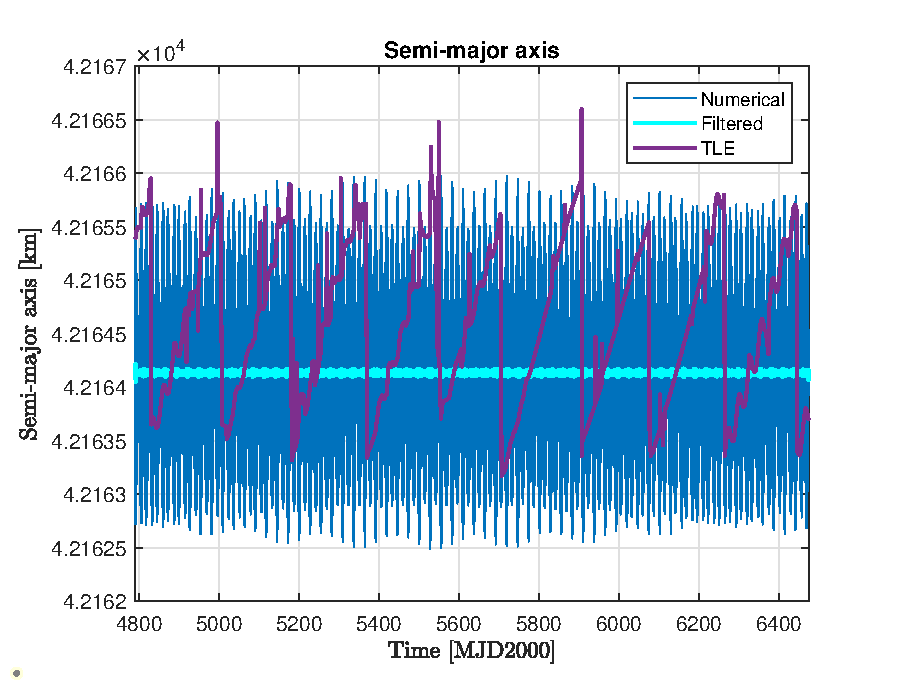
\includegraphics[width=\n\linewidth]{a_TLE.eps}
	\end{minipage}\hfill
	\begin{minipage}{0.48\linewidth}
		\centering
		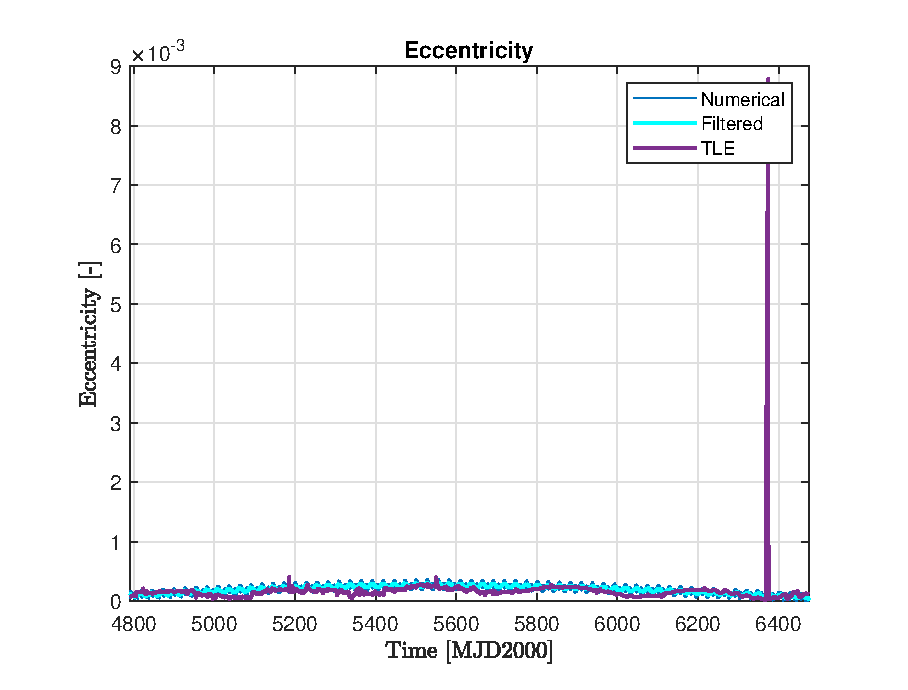
\includegraphics[width=\n\linewidth]{e_TLE.eps}
	\end{minipage}
	\vfill
	\begin{minipage}{0.48\linewidth}
		\centering
		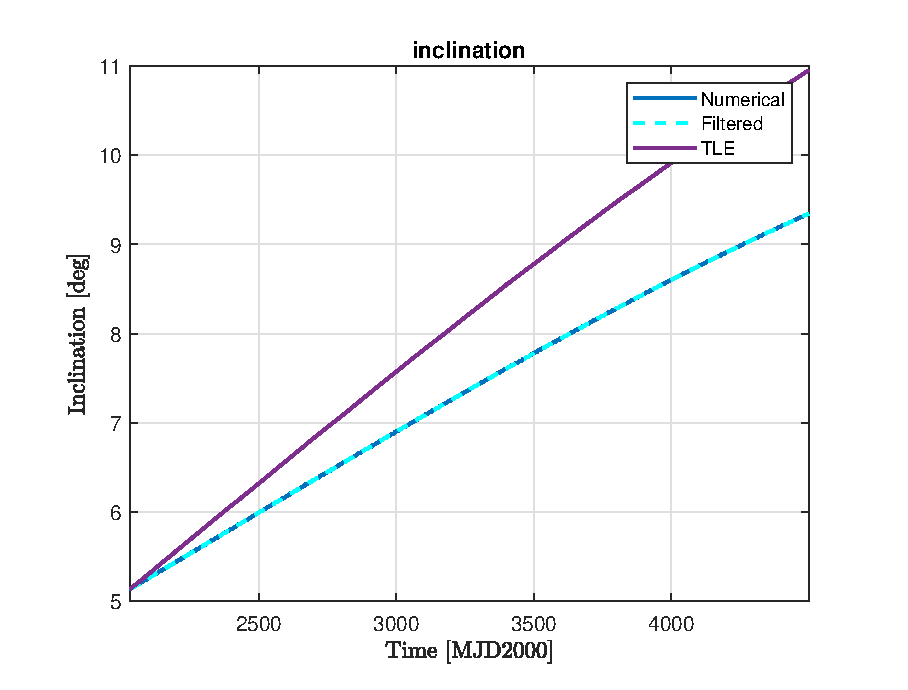
\includegraphics[width=\n\linewidth]{i_TLE.eps}
	\end{minipage}\hfill
	\begin{minipage}{0.48\linewidth}
		\centering
		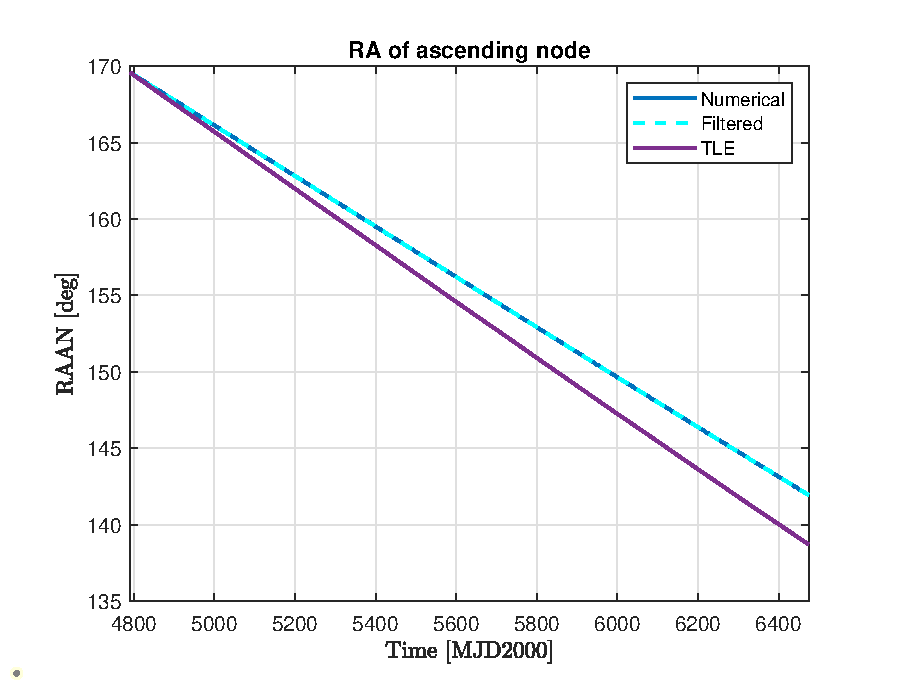
\includegraphics[width=\n\linewidth]{RAAN_TLE.eps}
	\end{minipage}
	\vfill
	\begin{minipage}{0.48\linewidth}
		\centering
		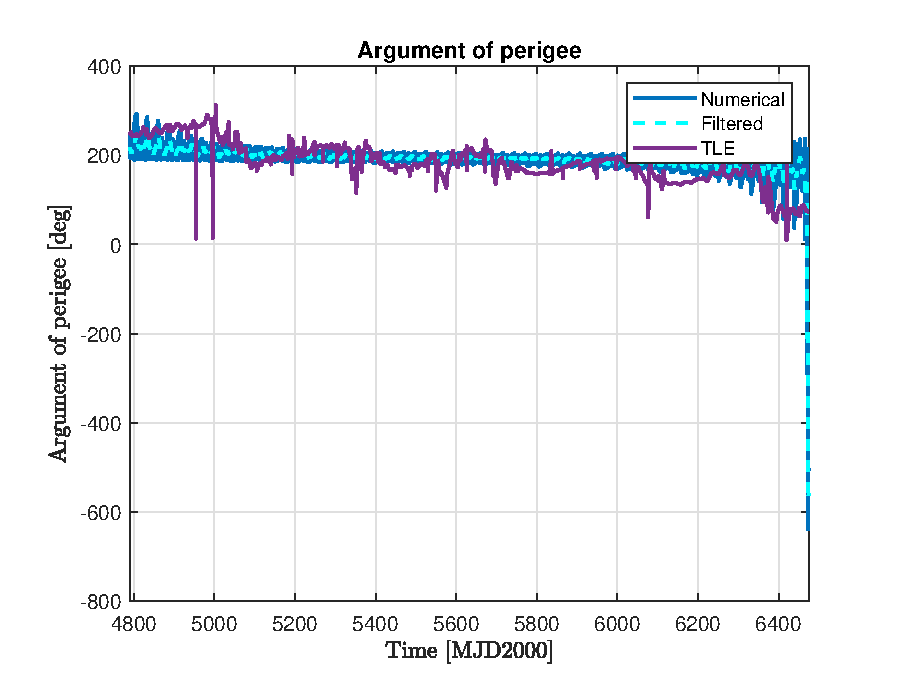
\includegraphics[width=\n\linewidth]{w_TLE.eps}
	\end{minipage}\hfill
	\begin{minipage}{0.48\linewidth}
		\centering
		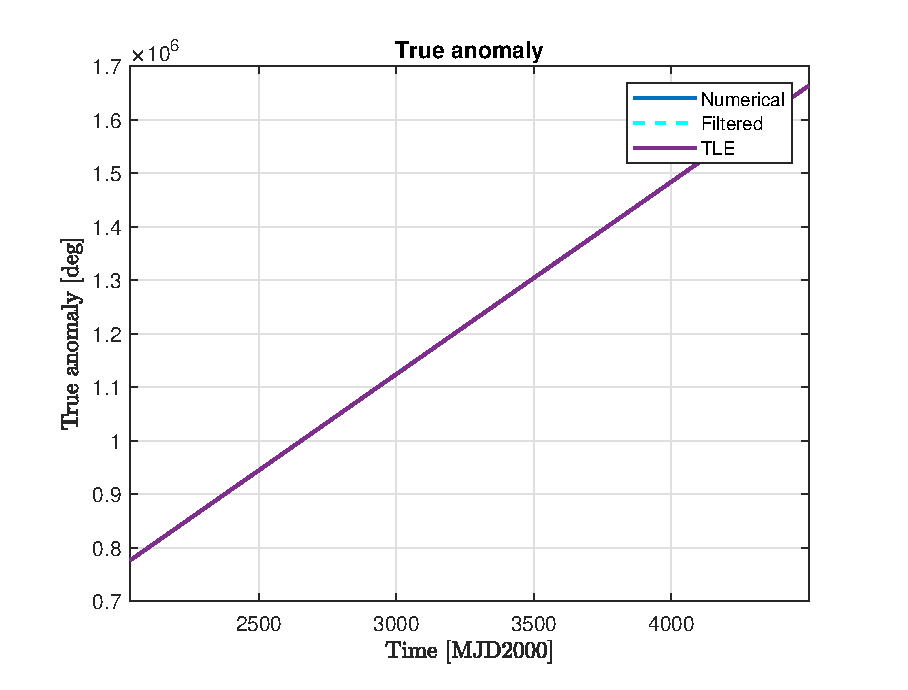
\includegraphics[width=\n\linewidth]{TA_TLE.eps}
	\end{minipage}
	\caption{Numerical, filtered and TLE data}
	\label{fig:comparison_figures}
\end{figure}

%---------------------------------------------------------------------------
% BIBLIOGRAFIA
%---------------------------------------------------------------------------

{\let\clearpage\relax
\vspace*{20mm}
\bibliography{bibliography}}

\end{document}